\documentclass[11pt]{article}

\usepackage[margin=1in]{geometry}
\usepackage{amsmath}
\usepackage{booktabs}
\usepackage{graphicx}
\usepackage{hyperref}
\IfFileExists{placeins.sty}{\usepackage{placeins}}{%
  \newcommand{\FloatBarrier}{\clearpage}}

\title{AthenaK CGL--Landau-Fluid Validation and MKS24 Analysis Note}
\author{}
\date{May 25, 2026}

\begin{document}
\maketitle

\section{Purpose}

This note integrates the illustrated validation report originally maintained
on branch \texttt{CGL-STS-LF} into the current
\texttt{feature/cgl-landau-fluid} implementation.  It documents the AthenaK
CGL--Landau-fluid (CGL--LF) heat-flux method, preserves its method-level
validation figures, and adds representative outputs from the reduced
Majeski--Kunz--Squire (2024, hereafter MKS24) analysis workflow.

The method-level results show that the implemented update follows the intended
finite-volume variable strategy and passes checks including a
one-dimensional oblique linear initial-value problem using the Squire et
al.\ Figure 17 background state.  The reduced nonlinear figures exercise
analysis and plotting paths only: they are not standard-resolution,
steady-state, or quantitative MKS24 reproduction results.  The current
execution and reference-admission status is maintained in
\texttt{docs/cgl\_lf\_mks24\_reproduction\_implementation\_plan.md} and in
the Sphinx CGL--LF validation guide.

\section{Conserved Variables}

The hyperbolic CGL system evolves total energy and the conserved anisotropy
variable
\begin{equation}
  A = \rho \log\left[
    \frac{p_\perp}{p_\parallel}
    \frac{\rho^2}{|B|^3}
  \right].
\end{equation}
The legacy array slot is still named \texttt{IMU}, with \texttt{IAN} used as an
alias in CGL code.  The Riemann solve remains in \(A\), which avoids the
small-\(|B|\) pathologies associated with evolving magnetic moment directly.

The LF STS operator temporarily changes only the interpretation of the
\texttt{IAN} slot:
\begin{equation}
  A \rightarrow \mu_B = \frac{p_\perp}{|B|}.
\end{equation}
The standard conserved-variable STS update then advances \((E,\mu_B)\) with the
LF flux divergence.  Immediately after the RKL2 stage, the EOS converts
\(\mu_B \rightarrow A\), and the normal CGL conserved-to-primitive recovery
restores \((p_\parallel,p_\perp)\).

In the current source tree the LF parabolic operator is owned by
\path{src/diffusion/cgl_landau_fluid.*}; the CGL state and constraint
logic are implemented in \path{src/eos/cgl_mhd.cpp} and
\path{src/eos/cgl_physics.hpp}.  The quantitative method tests use
\path{src/pgen/tests/cgl_landau_fluid.cpp}, while the reduced MKS24
initialization and history diagnostics use
\path{src/pgen/tests/cgl_lf_paper.cpp}.

\section{Landau-Fluid Closure}

The implemented closure uses the Snyder--Hammett--Dorland 3+1 heat fluxes,
\begin{align}
  q_\parallel &=
    -\chi_\parallel \rho \nabla_\parallel\left(\frac{p_\parallel}{\rho}\right),
  \\
  q_\perp &=
    -\chi_\perp \left[
      \rho \nabla_\parallel\left(\frac{p_\perp}{\rho}\right)
      - p_\perp\left(1-\frac{p_\perp}{p_\parallel}\right)
        \frac{\nabla_\parallel |B|}{|B|}
    \right],
\end{align}
with the finite-collision Squire et al. coefficients
\begin{equation}
  \chi_\perp =
    \frac{2c_\parallel^2}
      {\sqrt{2\pi}\,c_\parallel |k_\parallel| + \nu_{\rm eff}},
  \qquad
  \chi_\parallel =
    \frac{8c_\parallel^2}
      {\sqrt{8\pi}\,c_\parallel |k_\parallel|
        + (3\pi-8)\nu_{\rm eff}} .
\end{equation}
Here \(\nu_{\rm eff}\) is the background collision frequency plus any active
mirror/firehose limiter scattering at the face.  In the collisionless limit,
these reduce to
\(\chi_\perp=\sqrt{2/\pi}\,c_\parallel/|k_\parallel|\) and
\(\chi_\parallel=\sqrt{8/\pi}\,c_\parallel/|k_\parallel|\).
Here \texttt{lf\_k\_parallel} is the closure wavenumber \(|k_\parallel|\), not a
conductivity.  In local mode, \(c_\parallel=\sqrt{p_\parallel/\rho}\) is computed
from the live face state.  In background mode, only this prefactor is frozen to
\texttt{lf\_c\_parallel0}; all gradients and thermodynamic variables remain live.

The face fluxes coupled into STS are
\begin{equation}
  F_E^i = \hat{b}^i \left(q_\perp + \frac{1}{2}q_\parallel\right),
  \qquad
  F_{\mu_B}^i = \hat{b}^i \frac{q_\perp}{|B|}.
\end{equation}

\section{Heat-Flux Cap}

Following Squire et al. (2023), equations 3.1--3.2, the unlimited heat flux
\(q_L\) is capped as
\begin{equation}
  q = \frac{q_L q_{\max}}{q_{\max} + |q_L|}.
\end{equation}
The implemented caps are
\begin{equation}
  q_{\perp,\max} = \sqrt{\frac{2}{\pi}} c_\parallel p_\perp,
  \qquad
  q_{\parallel,\max} = \sqrt{\frac{8}{\pi}} c_\parallel p_\parallel.
\end{equation}
The cap is applied after computing the unlimited flux with the collision-aware
coefficient, so collisions and limiter scattering suppress the flux before the
smooth free-streaming bound is applied.

\section{Threshold Policy and Retained Diagnostics}

The current implementation separates backward-compatible operator tests from
MKS24 production definitions.  Existing method checks retain the default
oblique-firehose policy.  MKS24 decks set
\texttt{cgl\_firehose\_threshold = parallel}, selecting
\(\beta\Delta \leq -2\), together with the mirror threshold
\(\beta\Delta \geq 1\).  Hard-wall MKS24 decks additionally set
\texttt{limiter\_hardwall = true}; newly unstable primitive states are then
projected to the selected threshold while preserving
\(p_\perp + p_\parallel/2\), rather than relying on finite-rate limiter
relaxation to approximate an algebraic wall.

LF-enabled runs append persistent history counters for STS stages, floors,
non-finite and non-positive states, ordinary limiter occupancy, emergency
hard-bound crossings, heat-flux-cap activity, applied heat-flux
contractions, and hard-wall projection applications.  When enabled for
paper decks, \texttt{cgl\_lf\_record\_pressure\_work} also retains
explicit-RK-applied total and anisotropic CGL pressure-traction work.  Strict
validation rejects floors, invalid states, or emergency-bound crossings;
hard-wall projection activity is an expected model action, not by itself a
safety failure.

\section{Validation Workflow}

Generate the method-validation figures from the repository root with
\begin{verbatim}
python3 scripts/cgl_lf_workflow.py full --output-dir /path/to/full-bundle
\end{verbatim}
or with the compatibility command
\texttt{scripts/run\_cgl\_lf\_validation.sh}.  The driver writes an ignored
result bundle containing a manifest, readable summary, logs, histories,
machine-readable validation CSV files, and figures.  The five method figures
included below were regenerated from the retained passing bundle
\texttt{build-cgl-implementation/cgl\_lf\_runs/20260524-final-full-v2}.

Each test prints the measured value, reference value or error norm, tolerance,
and pass/fail status.  The plotted points are read from the same diagnostic CSV
files produced by the passing runs.

Generate reduced nonlinear diagnostic products with
\begin{verbatim}
python3 scripts/cgl_lf_workflow.py paper-convergence
python3 scripts/cgl_lf_workflow.py paper-analyze \
  --output-dir /path/to/paper-convergence-bundle
\end{verbatim}
The representative nonlinear figures below were regenerated with the current
analyzer from the retained passing
\texttt{20260525-paper-convergence-pressure-work-v1} bundle.  Its cases run
only through \(t=0.02\) on reduced grids and therefore test product plumbing,
not statistically saturated turbulence or paper agreement.

\section{Validation Problems and Tolerances}

\begin{table}[htbp]
\centering
\small
\begin{tabular}{p{0.32\textwidth}p{0.31\textwidth}p{0.27\textwidth}}
\toprule
Input & Purpose & Assertion \\
\midrule
\texttt{cgl\_transform\_check} & \(A \leftrightarrow \mu_B\) and primitive recovery
  & pass \\
\texttt{cgl\_lf\_quant\_parallel} & sinusoidal \(T_\parallel\) decay
  & final Fourier amplitude within 5\% of analytic decay \\
\texttt{cgl\_lf\_quant\_parallel}\\\texttt{\_collisional} & sinusoidal \(T_\parallel\) decay with \(\nu_{\rm c}>0\)
  & final Fourier amplitude within 7\% of finite-collision analytic decay \\
\texttt{cgl\_lf\_quant\_perp} & sinusoidal \(T_\perp\) decay
  & final Fourier amplitude within 5\% of analytic decay \\
\texttt{cgl\_lf\_quant\_perp}\\\texttt{\_collisional} & sinusoidal \(T_\perp\) decay with \(\nu_{\rm c}>0\)
  & final Fourier amplitude within 7\% of finite-collision analytic decay \\
\texttt{cgl\_lf\_quant\_grad\_b} & isolated \(\nabla_\parallel |B|\) term
  & RMS relative error below 10\%, positive response correlation \\
\texttt{cgl\_lf\_flux\_limiter} & equation 3.2 heat-flux cap
  & \(|q|\le q_{\max}\), sign preserved, update within 20\% \\
\texttt{cgl\_lf\_limiter}\\\texttt{\_heat\_flux\_suppression} & limiter-collision suppression of heat fluxes
  & active limiter scattering reduces the unlimited LF flux by more than 20x \\
\texttt{cgl\_lf\_limiter\_mirror} & mirror-biased admissibility stress
  & intermediate STS states finite, positive, and backup bounded \\
\texttt{cgl\_lf\_limiter\_firehose} & firehose-biased admissibility stress
  & intermediate STS states finite, positive, and backup bounded \\
\texttt{cgl\_lf\_field\_wave} & field-aligned LF wave reference
  & complex Fourier mode within 25\% of offline reference \\
\texttt{cgl\_lf\_paper\_oblique\_wave} & Figure 17 background, LF enabled
  & guard tolerance 40\%; observed errors \(<3\times10^{-6}\) \\
\texttt{cgl\_pure\_paper\_oblique\_wave} & Figure 17 background, no LF
  & guard tolerance 40\%; observed errors \(<3\times10^{-6}\) \\
\texttt{cgl\_pure\_paper\_eigen\_*} & exact pure-CGL Alfvén/slow/fast modes
  & all tracked Fourier components within 7.5\% \\
\texttt{cgl\_lf\_paper\_eigen\_*} & exact CGL--LF Alfvén/slow/fast modes
  & all tracked Fourier components within 7.5\% \\
\bottomrule
\end{tabular}
\end{table}

\section{Quantitative Results}

\begin{figure}[htbp]
\centering
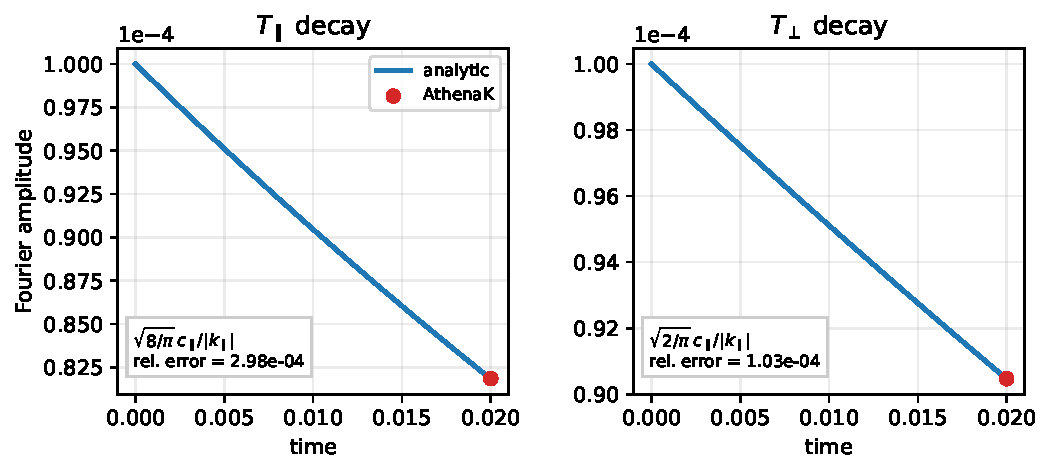
\includegraphics[width=0.92\textwidth]{figures/cgl_lf_decay.pdf}
\caption{Constant-coefficient decay tests.  The \(T_\parallel\) case uses
\(\chi_\parallel=\sqrt{8/\pi}c_\parallel/|k_\parallel|\); the \(T_\perp\) case
uses \(\chi_\perp=\sqrt{2/\pi}c_\parallel/|k_\parallel|\).  The red point is
the final AthenaK Fourier amplitude and the blue curve is the analytic
constant-coefficient decay.}
\end{figure}

\begin{figure}[htbp]
\centering
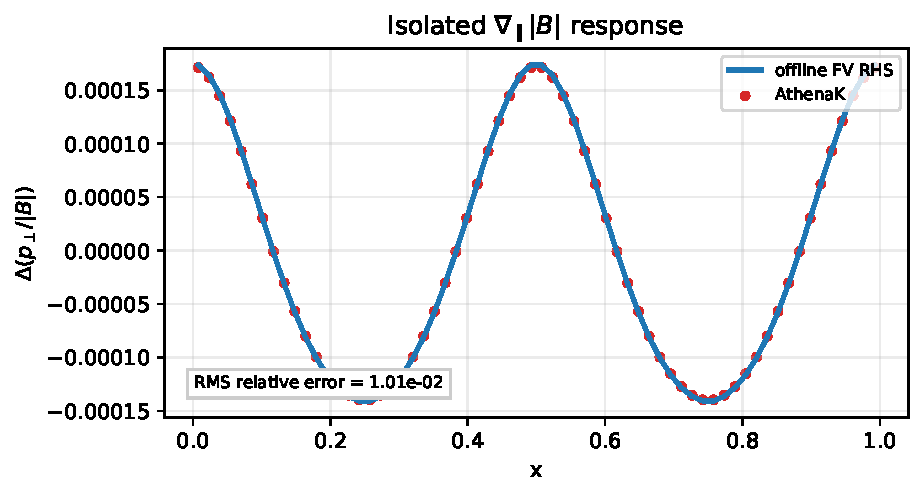
\includegraphics[width=0.78\textwidth]{figures/cgl_lf_grad_b.pdf}
\caption{Isolated \(\nabla_\parallel |B|\) term in the perpendicular heat flux.
The initial thermal gradients are zero; the plotted response is the short-time
change in \(p_\perp/|B|\) compared with an offline finite-volume reconstruction
of the initial LF RHS.}
\end{figure}

\begin{figure}[htbp]
\centering
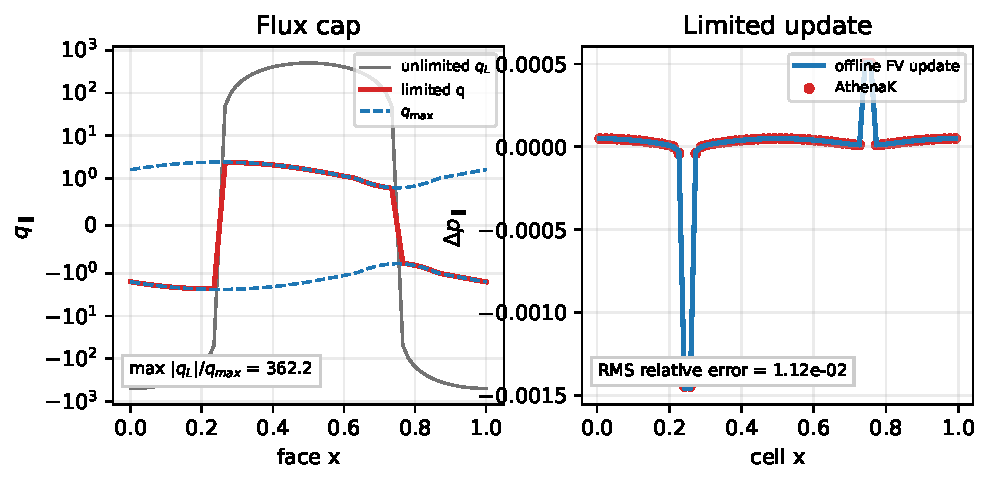
\includegraphics[width=0.92\textwidth]{figures/cgl_lf_flux_limiter.pdf}
\caption{Heat-flux limiter test.  The left panel shows the unlimited
\(q_{\parallel,L}\), the capped \(q_\parallel\), and \(\pm q_{\parallel,\max}\).
The right panel checks that the pressure update produced by the limited flux
matches the offline finite-volume update.}
\end{figure}

\begin{figure}[htbp]
\centering
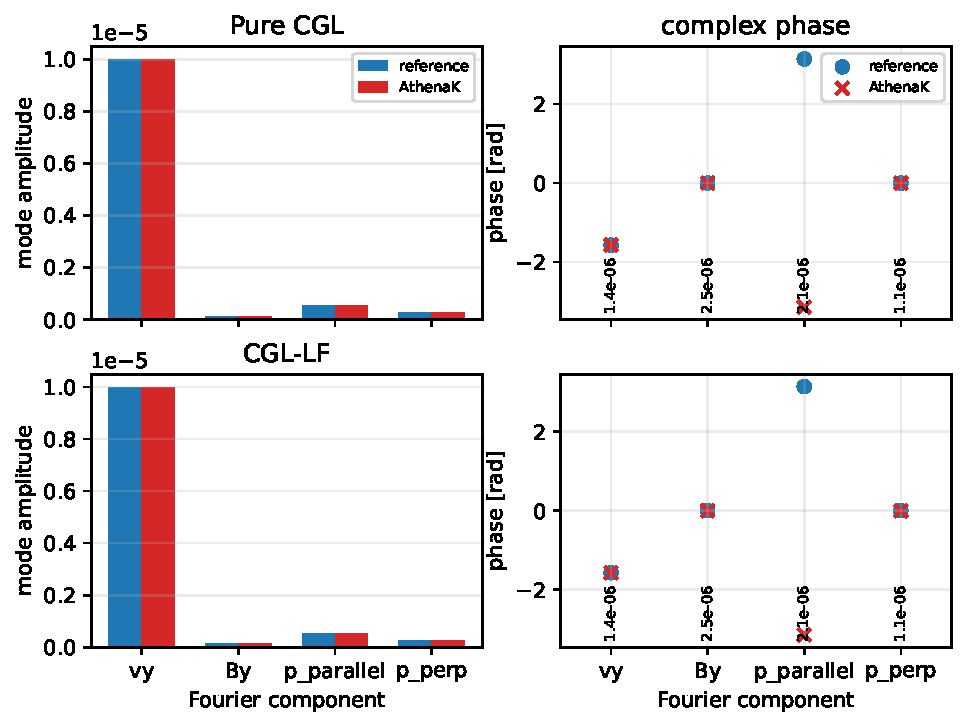
\includegraphics[width=0.92\textwidth]{figures/cgl_lf_paper_oblique_wave.pdf}
\caption{Figure 17-style oblique linear initial-value check.  The plotted quantities are
the final complex Fourier amplitudes of \(u_y\), \(B_y\), \(p_\parallel\), and
\(p_\perp\) for the pure-CGL and CGL--LF inputs, compared with the offline
linearized initial-value reference used by the quantitative pgen.  The vertical phase-panel
labels are per-variable relative errors.}
\end{figure}
\FloatBarrier

\section{Figure 17-Style Linear Initial-Value Check}

The paper-style inputs use the Figure 17 background
\begin{equation}
  \rho_0 = 1,\quad p_{\parallel 0}=p_{\perp 0}=5,\quad
  u_0=0,\quad B_0=(1,\sqrt{2},0.5),\quad k=2\pi \hat{x},
  \quad kL=|k|.
\end{equation}
The test initializes a small transverse velocity perturbation, not a CGL
eigenmode, and compares the
final complex Fourier amplitudes of \(u_y\), \(B_y\), \(p_\parallel\), and
\(p_\perp\) against an offline linearized CGL--LF initial-value reference integrated with the
same background state and closure coefficients.  Two inputs are provided: one
with the LF heat flux enabled and one with pure CGL.  This checks the same
method class as the Appendix A.2/Figure 17 linear-wave convergence problem.

\section{Figure 17-Style Eigenmode Checks}

The validation suite now also includes exact eigenmode initializations for the
Alfvén, slow-like, and fast-like positive-frequency branches of the same
linearized Figure 17 system.  The script
\texttt{scripts/generate\_cgl\_lf\_eigenmode\_inputs.py} constructs the
linear CGL or CGL--LF matrix for the AthenaK variables
\((\rho,u_x,u_y,u_z,B_y,B_z,p_\parallel,p_\perp)\), diagonalizes it, normalizes
the selected eigenvectors, and writes their complex amplitudes and eigenvalues
into AthenaK input files.  The pgen initializes
\(\mathrm{Re}[\delta U_k \exp(ikx)]\) and compares the final Fourier mode with
\(\delta U_k\exp(\lambda t)\), where \(\lambda\) is the supplied eigenvalue.
These inputs are the direct replacement for using a single transverse-velocity
seed as a proxy for the Squire/Jono linear-wave comparisons.

\begin{figure}[htbp]
\centering
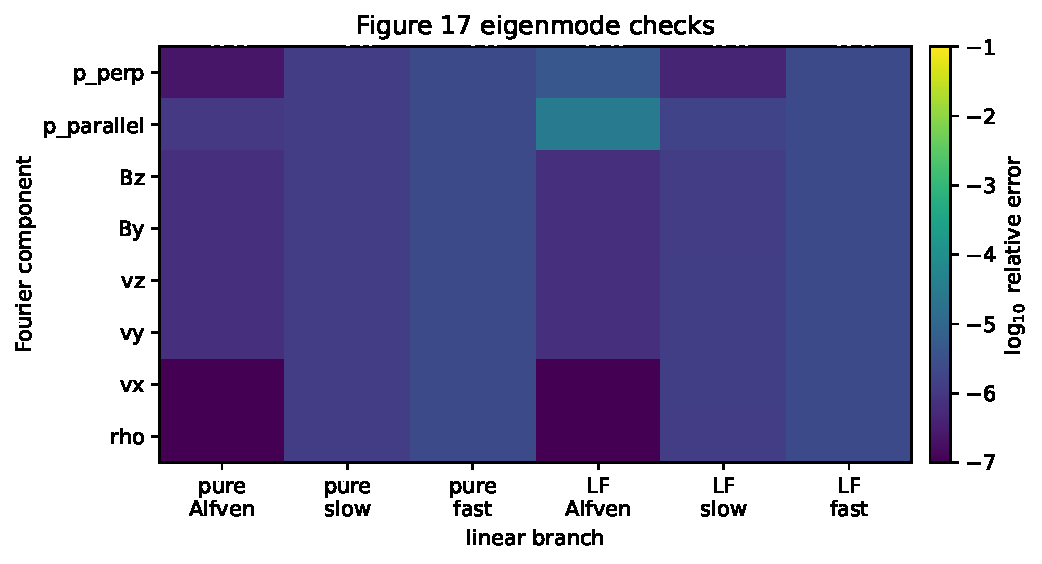
\includegraphics[width=0.92\textwidth]{figures/cgl_lf_paper_eigenmodes.pdf}
\caption{Exact eigenmode checks on the Figure 17 background.  Each column is a
pure-CGL or CGL--LF Alfvén, slow-like, or fast-like positive-frequency branch.
The color scale shows the complex Fourier relative error in each primitive or
magnetic component after a short AthenaK evolution compared with the supplied
linear eigenmode prediction \(\delta U_k\exp(\lambda t)\).  The white numbers
give the maximum tracked-component error in each branch.}
\end{figure}
\FloatBarrier

\section{Reduced MKS24-Oriented Analysis Products}

The \texttt{paper-convergence} workflow supplies short, reduced forced
turbulence bundles used to validate nonlinear diagnostics and rendering.  The
figures in this section use the current analyzer on retained snapshots from
\texttt{20260525-paper-convergence-pressure-work-v1}.  The bundle contains
three resolution-path cases and heat-flux/policy variants, all with clean LF
safety diagnostics.  Because these cases terminate at \(t=0.02\), their
curves must not be interpreted as steady turbulent spectra or MKS24
comparisons.

\begin{figure}[htbp]
\centering
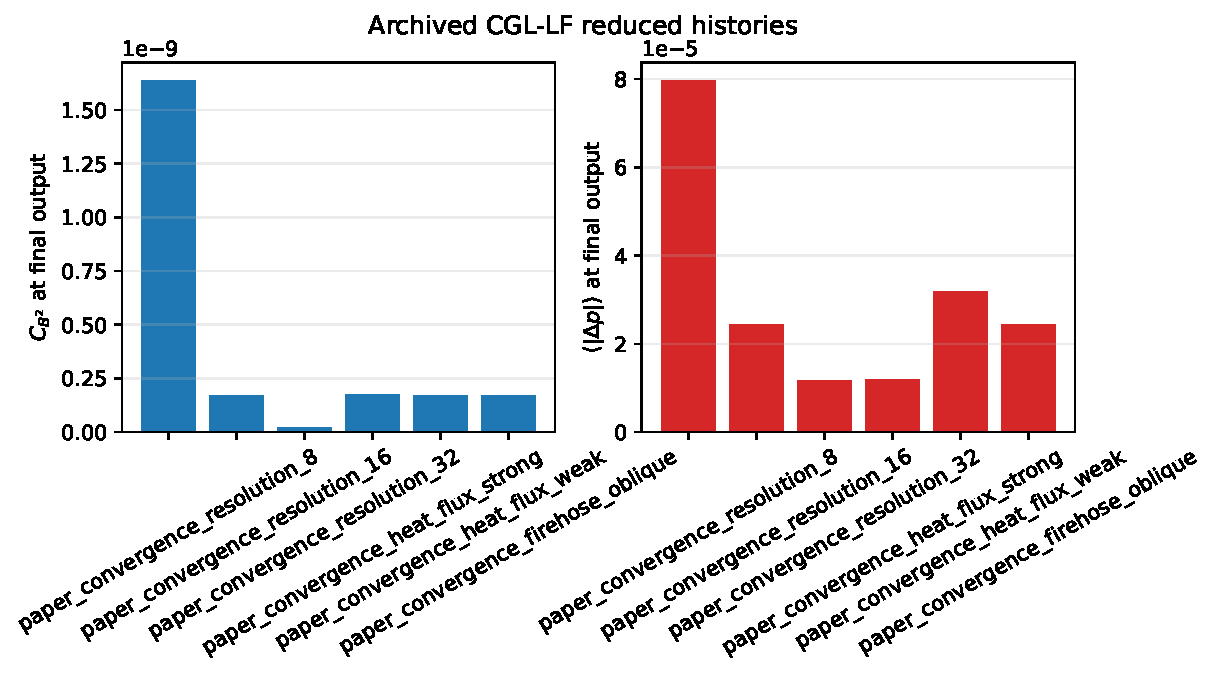
\includegraphics[width=0.94\textwidth]{figures/cgl_lf_paper_history_summary.pdf}
\caption{Reduced history-product rendering for the nonlinear analysis path.
The plotted global summaries verify ingestion of archived history data across
the reduced case matrix; they do not establish converged physical trends.}
\end{figure}

\begin{figure}[htbp]
\centering
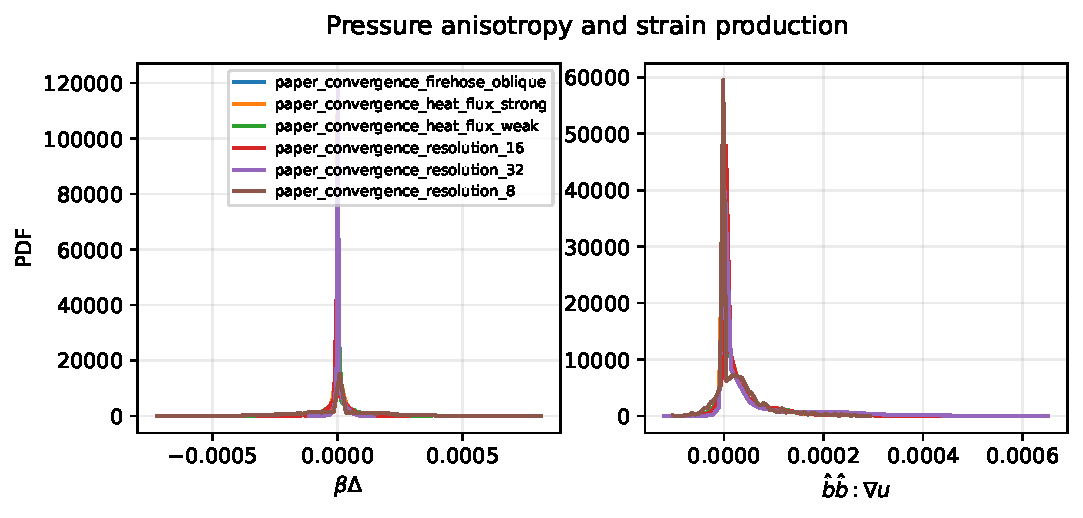
\includegraphics[width=0.94\textwidth]{figures/cgl_lf_paper_pdfs.pdf}
\caption{Reduced pressure-anisotropy and local-strain PDF rendering.  These
products expose \(\beta\Delta\) and
\(\hat{\boldsymbol b}\hat{\boldsymbol b}:\nabla\boldsymbol u\) for later
panel comparisons once authorized statistically useful runs exist.}
\end{figure}

\begin{figure}[htbp]
\centering
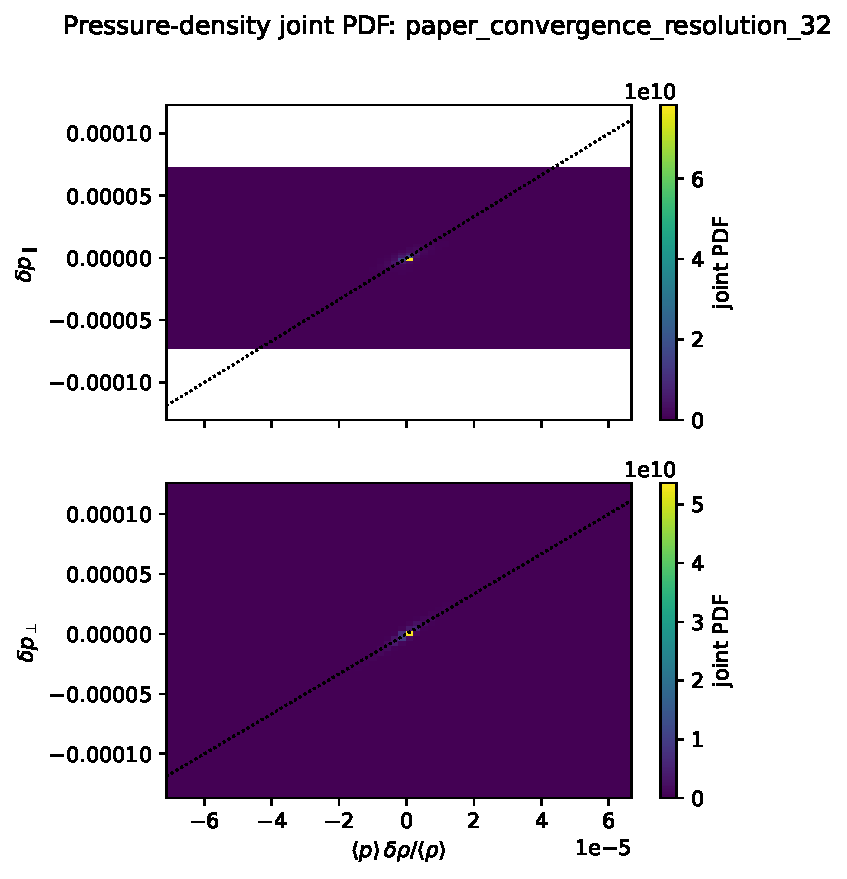
\includegraphics[width=0.72\textwidth]{figures/cgl_lf_paper_pressure_density_resolution_32.pdf}
\caption{Representative Figure 2(a)-coordinate joint-PDF diagnostic from the
\(32\times32\times64\) reduced case.  The analyzer now emits
\(\langle p\rangle\delta\rho/\langle\rho\rangle\) versus
\(\delta p_\parallel\) and \(\delta p_\perp\).  The admitted digitized MKS24
surface route is separate from this reduced simulation output and requires a
matching standard case.}
\end{figure}

\begin{figure}[htbp]
\centering
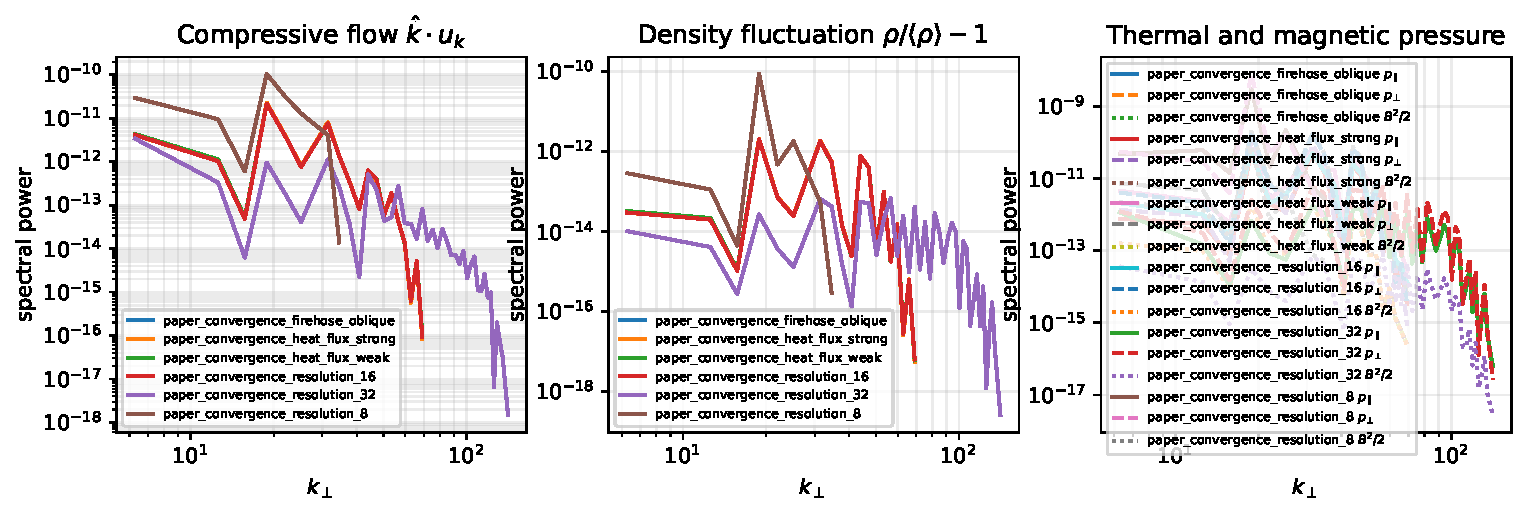
\includegraphics[width=0.94\textwidth]{figures/cgl_lf_paper_compressive_pressure_spectra.pdf}
\caption{Current reduced rendering of the Figure 3/4(b)/6(a)-oriented
spectral fields: compressive velocity projection, normalized density
fluctuation, and thermal/magnetic-pressure products.  Their plotted MKS24
absolute ordinates remain excluded from reference comparison until an
external discrete Fourier-normalization mapping or original numeric data are
available.}
\end{figure}

\begin{figure}[htbp]
\centering
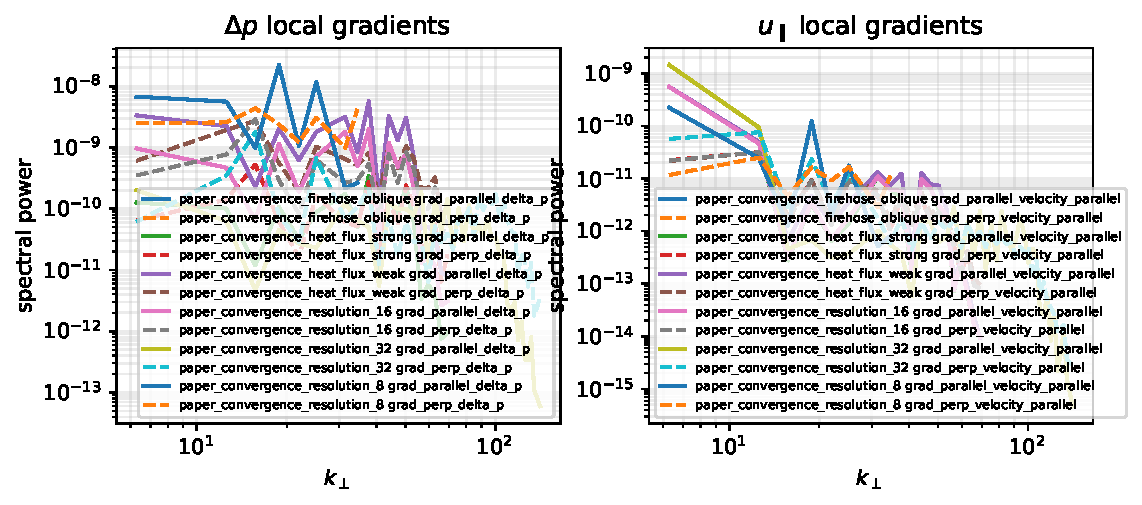
\includegraphics[width=0.94\textwidth]{figures/cgl_lf_paper_projected_spectra.pdf}
\caption{Projected pressure-anisotropy and velocity-gradient spectrum
products from the reduced bundle.  These are diagnostic-product checks and
not admitted absolute-ordinate paper comparisons.}
\end{figure}

\begin{figure}[htbp]
\centering
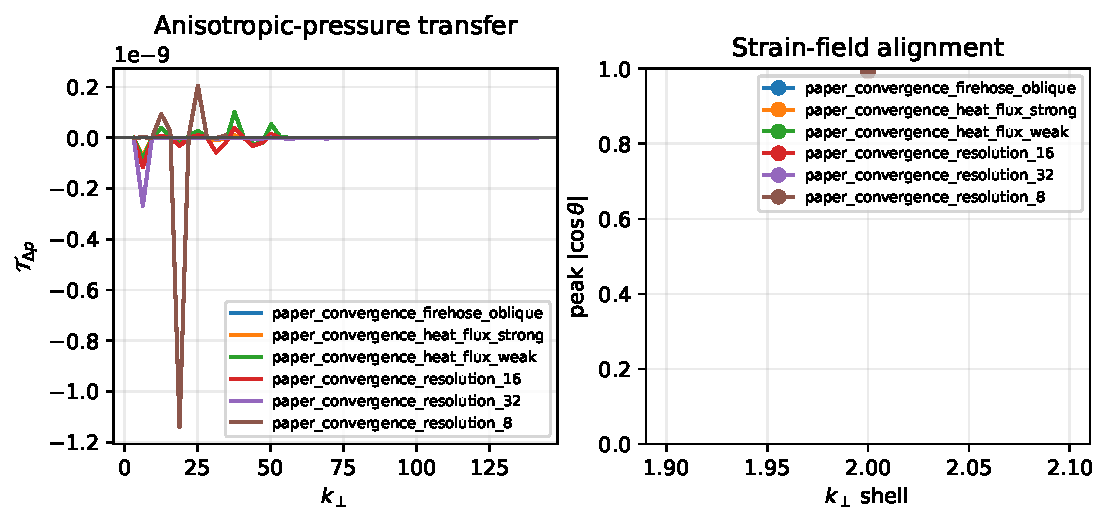
\includegraphics[width=0.94\textwidth]{figures/cgl_lf_paper_transfer_alignment.pdf}
\caption{Pressure-stress transfer and alignment-product rendering.  The
analyzer supports the dimensionless MKS24-normalized transfer comparison and
selected-shell or peak-alignment comparisons when supplied with
provenance-qualified references and matching executed cases.}
\end{figure}

\begin{figure}[htbp]
\centering
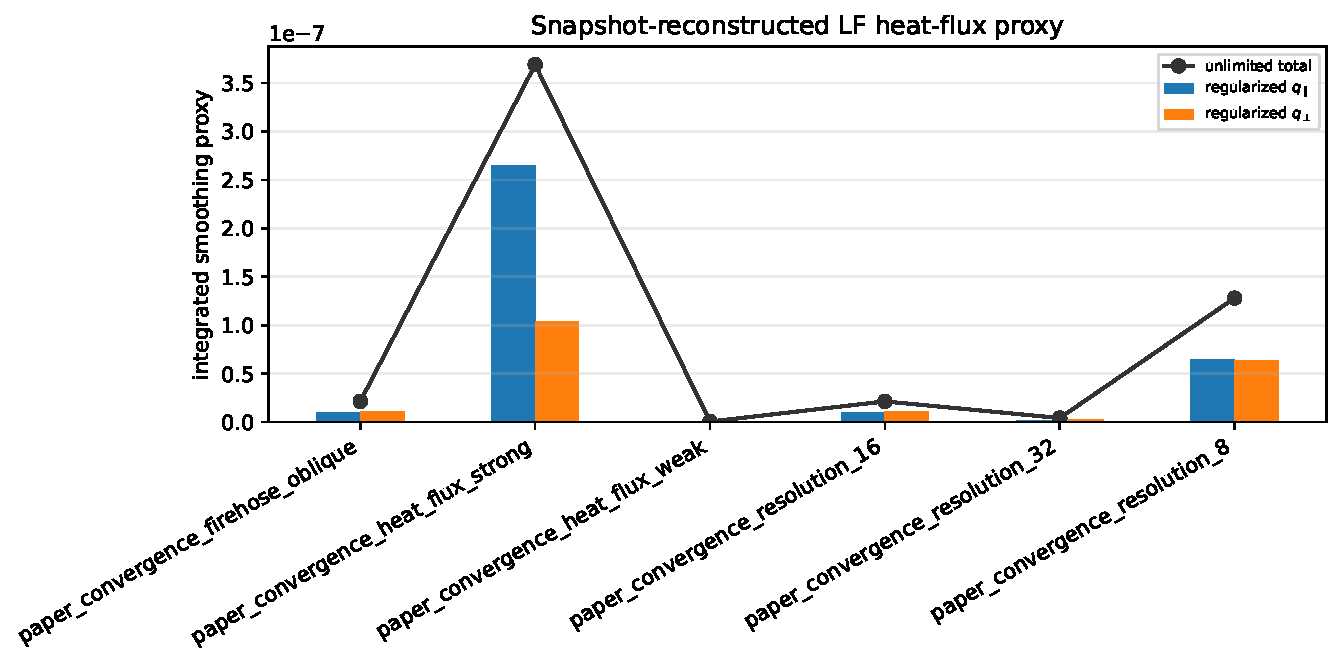
\includegraphics[width=0.94\textwidth]{figures/cgl_lf_paper_heat_flux_proxy.pdf}
\caption{Snapshot-reconstructed heat-flux smoothing proxy for reduced cases.
It is useful for interpretation of retained snapshots, but is not the
applied finite-volume heat-flux contraction or a total energy closure.}
\end{figure}

\begin{figure}[htbp]
\centering
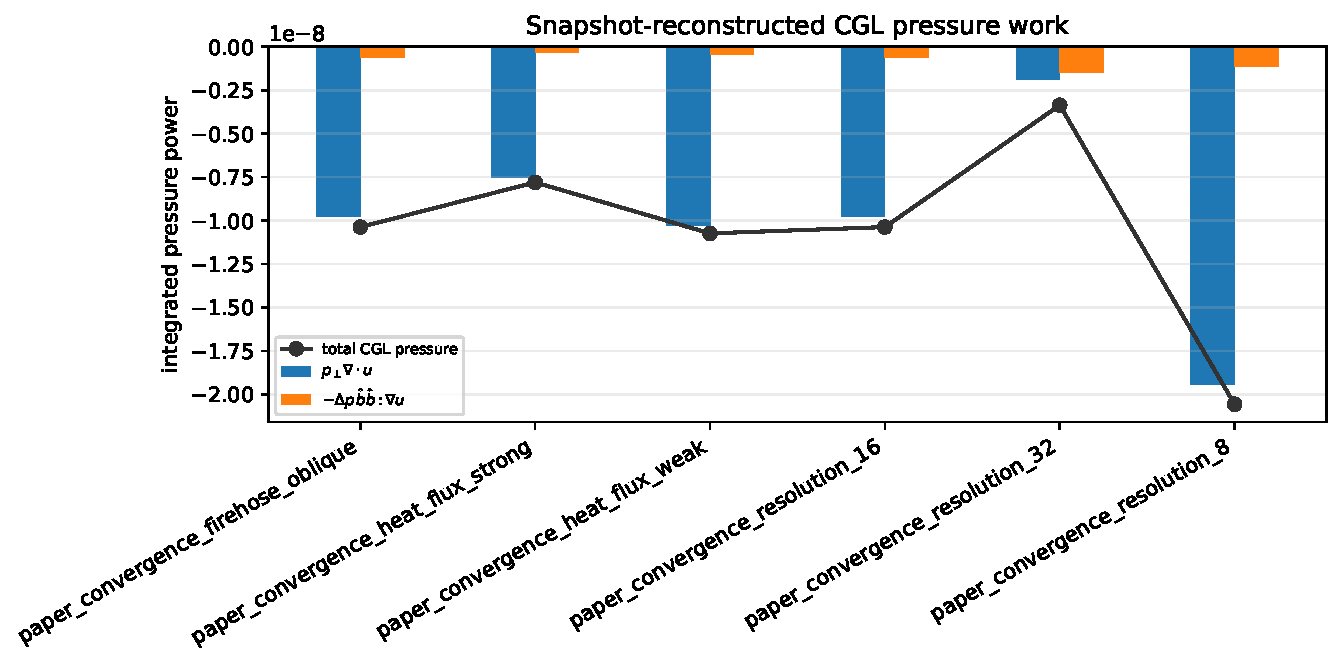
\includegraphics[width=0.94\textwidth]{figures/cgl_lf_paper_pressure_work.pdf}
\caption{Snapshot-derived CGL pressure-work decomposition, including the
anisotropic stress contribution checked against direct pressure transfer.
Paper decks also retain applied pressure-traction ledger histories; neither
the reduced snapshot plot nor an unevaluated standard deck establishes a
production result.}
\end{figure}
\FloatBarrier

\section{MKS24 Reproduction Boundary}

The current branch defines guarded standard, limiter-frequency, heat-flux,
compressive, and scale-separation workflows and supports
checksum/uncertainty-qualified external reference comparisons.  The admitted
published reference products presently include Figure 2(a) transformed
sampled surfaces, Figure 2(b) histories, normalized Figure 4(a) PDFs,
normalized Figure 5(b) eddy scales, dimensionless Figure 7 transfer ratios,
Figure 8 selected-shell alignment PDFs, Figure 9 and Figure 11/12 alignment
curves, and Figure 13(b),(d) dimensionless products.

Remaining absolute spectral or strain ordinate panels are intentionally not
admitted: the paper and cited donor source define shell spectra and plotted
units but do not state the discrete Fourier normalization needed to map
absolute digitized ordinates into AthenaK products.  Those panels require
author/archive numeric data, donor diagnostic code, or an explicit
normalization statement.  Production executions and quantitative MKS24
simulation-to-reference comparisons additionally require explicit
authorization; none is claimed by this note.

\section{Build and Runtime Status}

The imported method figures come from a passing local \texttt{full} workflow
bundle.  The reduced nonlinear figures come from a passing
\texttt{paper-convergence} bundle reanalyzed with the current plotting code.
Warning-strict Sphinx documentation and this \LaTeX{} build are checked when
the report is updated.  Production/statistical and paper-reference comparison
gates remain outside this method-document build.

\begin{thebibliography}{9}
\bibitem{Squire2023}
J. Squire et al.,
\emph{Pressure anisotropy and viscous heating in weakly collisional plasma
turbulence},
\href{https://arxiv.org/abs/2303.00468}{arXiv:2303.00468}, 2023.

\bibitem{Majeski2024}
S. Majeski, M. W. Kunz, and J. Squire,
\emph{Self-organization in collisionless, high-\(\beta\) turbulence},
\href{https://arxiv.org/abs/2405.02418}{arXiv:2405.02418}, 2024.
\end{thebibliography}

\end{document}
